\documentclass{izpit}

\begin{document}

%==========================================================================
%               Sem vpisi podatke o izpitu
%=========================================================================
\FRACTIONSIMPLIFY{24}{1}{\skupnotock}{\nepomembno}%Sem vpiši (v polje trenutno {60}) skupno število točk, da paket naračuna kriterij ocenjevanj
\izpit[ucilnica = RAZRED, naloge = 3]%ucilnica RAZRED, lahko se sedezni red, ime in priimek, maturitetni
{Eksponentna in logaritemska funkcija}{9. 5. 2024}{Čas pisanja je 45 minut.\\ Možno je doseči $\skupnotock$ točk.\\ Veliko uspeha!}
%==========================================================================
%               Nepomembno - Preskoči
%==========================================================================
\MAX{0.1}{0}{\tempepsilon}%shranimo epsilon... ne gre trik z ulomkom zato max
\MULTIPLY{\skupnotock}{0.89}{\odlicno}
\MULTIPLY{\skupnotock}{0.76}{\pravdobro}
\MULTIPLY{\skupnotock}{0.62}{\dobro}
\MULTIPLY{\skupnotock}{0.5}{\zadostno}
\ADD{\dobro}{\tempepsilon}{\dobroplus}
\ADD{\pravdobro}{\tempepsilon}{\pravdobroplus}
\ADD{\odlicno}{\tempepsilon}{\odlicnoplus}
\ROUND[1]{\dobroplus}{\dobroplus}
\ROUND[1]{\pravdobroplus}{\pravdobroplus}
\ROUND[1]{\odlicnoplus}{\odlicnoplus}
\ROUND[1]{\zadostno}{\zadostno}
\ROUND[1]{\dobro}{\dobro}
\ROUND[1]{\pravdobro}{\pravdobro}
\ROUND[1]{\odlicno}{\odlicno}\begin{small}
 \PlaceText{100mm}{33mm}{\begin{tabular}{ll}
    \multicolumn{2}{c}{\textbf{Kriterij ocenjevanja}} \\[0.5ex]
    Ocena & Tocke \\ \hline
    zadostno & $12 - 15$ \\
    dobro & $16 - 18$ \\
    prav dobro & $19 - 21$ \\
    odlicno & $22$--
  \end{tabular}}\end{small}
 \ifthenelse{\boolean{@maturitetni}}{\newpage}%TO JE ZELO GRDA KODA a ker ne gre kriterij v class ni druge moznosti
%==========================================================================
%               Sem vpisi naloge
%   za dodatek koordinatnega sistema daj pod navodila naloge \dodatek{\[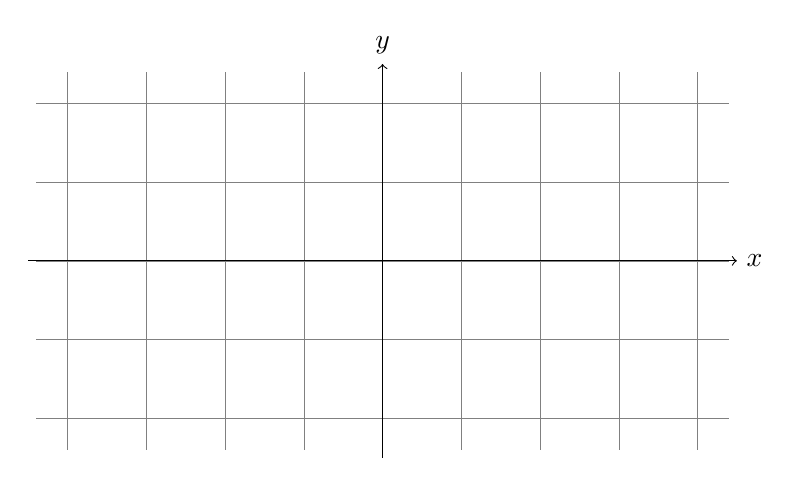
\begin{tikzpicture}
        \draw[help lines,step=1cm] (-4.4,-2.4) grid (4.4,2.4);
        \draw[->] (-4.5,0) -- (4.5,0) node[right] {$x$};
        \draw[->] (0,-2.5) -- (0,2.5) node[above] {$y$};
\end{tikzpicture}\]}
%   oz. za kompleksno ravnino \dodatek\[\begin{tikzpicture}
        \draw[help lines,step=1cm] (-4.4,-2.4) grid (4.4,2.4);
        \draw[->] (-4.5,0) -- (4.5,0) node[right] {$Re$};
        \draw[->] (0,-2.5) -- (0,2.5) node[above] {$Im$};
\end{tikzpicture}\]
%==========================================================================

\naloga[\tocke{6}]
  Funkciji $f(x)=\log_2{\left(x+2\right)}-1$ določi definicisko območje (računsko) in jo nariši. Napiši tri točke, ki ležijo na grafu te funkciji in jih na grafu tudi označi. Nato funkciji $f(x)$ določi inverzno funkcijo $f^{-1}(x)$.
  \dodatek{\[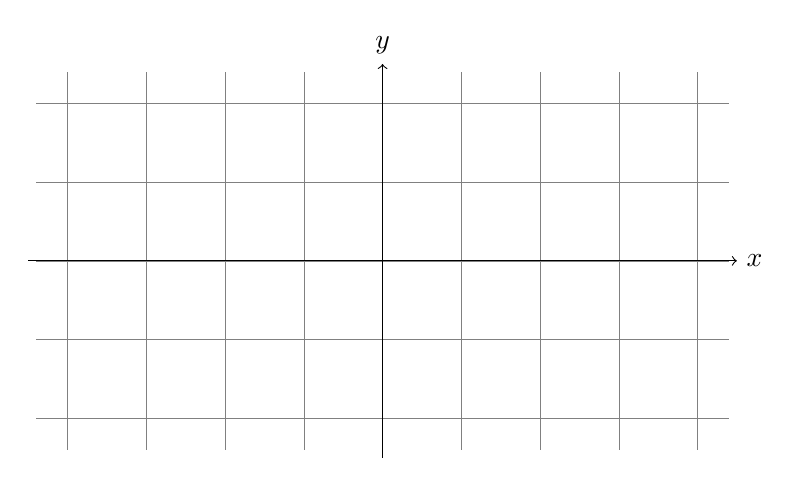
\begin{tikzpicture}
        \draw[help lines,step=1cm] (-4.4,-2.4) grid (4.4,2.4);
        \draw[->] (-4.5,0) -- (4.5,0) node[right] {$x$};
        \draw[->] (0,-2.5) -- (0,2.5) node[above] {$y$};
\end{tikzpicture}\]}


\naloga[\tocke{12}]
  Reši enačbe:
  \podnaloga[\tocke{4}]
  \[2^{2x-1}+2^x=4\]
  \prostor[1]

  \podnaloga[\tocke{4}]
  \[2^{x+1}+3^{x-1}=2^{x-1}+3^x\]
  \prostor[1]

  \podnaloga[\tocke{4}]
  \[\log_2{\left(5-3x\right)}+\log_2{\left(9-x\right)}-4=0\]
  \prostor[1]

\naloga*[\tocke{6}]
  Izračunaj $\log_9{8}\cdot\log_4{81}+\ln{\sqrt{e}}+\log_3{\frac{\sqrt{3}}{3}}-10^{\log{2}}$.
  \prostor[1]


\end{document}